\documentclass[11pt]{article}

\usepackage[utf8]{inputenc}
\usepackage[margin=1.2in]{geometry}
\usepackage{mathtools}
\usepackage{amsthm}
\usepackage{amssymb}
\usepackage[linesnumbered,ruled,vlined]{algorithm2e}
\usepackage{graphicx}
\usepackage{epsfig}
\usepackage{float}
\usepackage[hidelinks, colorlinks=false]{hyperref}
\usepackage{tabularx}

\renewcommand{\thealgocf}{} % prevents Algorithms from being numbered

\title{Machine Learning Final Project: Airbnb Pricing}
\author{Abhay Kasturia [MSCS, fourth semester] ~\\ Nakul Camasamudram [MSCS, third semester] ~\\ Philip Parker [MSCS, third semester]}
\date{}

\begin{document}
	\maketitle
    
	\section{Introduction}
    % Provide a short background of the project (e.g., what kind of question is to be answered with this dataset). Provide a short non-technical summary of your analysis.
    	\paragraph{}
        	Airbnb is a popular online company through which property owners (known as ``hosts") can short-term rent their spaces to consumers as an alternative to hotels. A host must decide what daily price to charge for his or her space based on its amenities. Clearly, with data on listed properties, this can be considered as a regression problem for supervised machine learning. However, many real estate datasets include categorical location features with large numbers of levels - which can pose computational difficulties for some methods. With that in mind, in this project we investigate two questions:
			\begin{description}
            	\item[(1)] To what degree can supervised machine learning techniques be used to assist an Airbnb host in determining an appropriate listing price for their property?
                \item[(2)] For Airbnb data, can the categorical feature of ``neighborhood" be replaced with a continuous feature of driving distance to a geographic point of interest (e.g., an airport) and have comparable results?
            \end{description}
            
		\paragraph{}
            To address these questions, we use data collected on Boston Airbnb property listings by the Inside Airbnb project$^{[1]}$. Our analysis shows that (1) while not outstanding, the performance of the machine learning techniques is useful for an Airbnb host, and (2) replacing the ``neighborhood" feature with either driving distance to the Boston airport or to the Boston downtown results in nearly identical performance.
            
                  
    \section{Methodology}
    % Summarize the methodology used, and use mathematical formulae and notation when appropriate
  
 		\subsection{Experimental Design}
            \paragraph{}
            	In order to perform our analysis, we conduct the following steps:
                
             \paragraph{(1) Collect Data:}
             	For our base data, we use the Airbnb property listing data collected by the Inside Airbnb project for the city of Boston which is available for public download$^{[2]}$. The data contains 4870 rows and 96 columns.
             	
             \paragraph{(2) Select Features:}
             	At this point, our data contains 96 features, many of which are textual data that are inappropriate for use in this analysis. After review, we select the following 17 relevant features for consideration:
                \begin{description}
                	\item[\textit{host\_is\_superhost}] (categorical -\textit{YES/NO}) whether the host is an ``Airbnb Superhost"
                    
                    \item[\textit{host\_identity\_verified}] (categorical - \textit{YES/NO}) whether Airbnb has verified the identity of the host 
                    
                    \item[\textit{neighborhood}] (categorical - \textit{25 levels}) the neighborhood that the property is in
                    
                    \item[\textit{property\_type}] (categorical - \textit{17 levels}) the type of property 
                    
                    \item[\textit{room\_type}] (categorical - \textit{Entire home/Private room/Shared room} ) the type of room 
                    
                    \item[\textit{accommodates}] (continuous) the number of people the property can hold
                    
                    \item[\textit{bathrooms}] (continuous) the number of bathrooms the property has
                    
                    \item[\textit{bedrooms}] (continuous) the number of bedrooms the property has
                    
                    \item[\textit{beds}] (continuous) the number of beds the property has
                    
                    \item[\textit{bed\_type}] (categorical - \textit{Airbed/Couch/Futon/Pull-out Sofa/Real Bed}) the type of bed 
                    
                    \item[\textit{guests\_included}] (continuous) the number of guests allowed
                    
                    \item[\textit{minimum\_nights}] (continuous) the minimum number of nights for a reservation
                    
                    \item[\textit{number\_of\_reviews}] (continuous) the number of reviews a property has received
                    
                    \item[\textit{instant\_bookable}] (categorical - \textit{YES/NO}) whether the property can be reserved through the Airbnb instant booking interface 
                    
                    \item[\textit{is\_business\_travel\_ready}] (categorical - \textit{YES/NO}) whether the property is considered ``business travel ready" 
                    
                    \item[\textit{cancellation\_policy}] (categorical - \textit{flexible/moderate/strict/super\_strict\_30/super\_strict\_60}) the strictness of the cancellation policy is
                    
                    \item[\textit{*price*}] (continuous) the feature we are regressing on: the daily price of the property in dollars
	
                \end{description}
             
             \paragraph{(3) Handle Missing Values:}
             	After selecting which features to consider, there are 14 rows which contain missing values. This is very small relative to the 4870 total rows in the dataset, so we can remove them without concern about the effect that will have on the analysis.
                
             \paragraph{(4) Handle Outliers:}
             	In our analysis of the data, we find that there are a number of outliers with listing prices extremely greater than the median. We make the decision to exclude rows with prices above the 95th percentile. This results in the removal of 240 outliers.
                
             \paragraph{(5) Create Data Transformations:}
             	We would like to see if we can replace the categorical feature of ``neighborhood" with a continuous feature of driving distance to a geographic point of interest. For this project, we create three transformations of the data to investigate:    
                \begin{description}
                	\item[1.] ``neighborhood" feature replaced with driving distance to Logan International Airport
                    \item[2.] ``neighborhood" feature replaced with driving distance to Downtown Crossing Station
                    \item[3.]  ``neighborhood" feature replaced with both of these. 
                \end{description}
	In order to create these transformations, we use the R package ``gmapsdistance" to obtain the driving distance from the neighborhood to the point of interest$^{[3]}$. Also a set of datasets are created having dummy variables for categorical data, for linear regression.
             
             
             \paragraph{(6) Separate Training/Model Selection/Validation Datasets:}
             	For the supervised machine learning task, we need to separate our data into training, model selection, and validation sets. For each data transformation, we randomly allocate 55\% of the rows for training, 15\% for model selection, 15\% for a first validation set, and 15\% for a second validation set (see figure). The allocation is performed such that the rows selected for each dataset are identical for each transformation.
                
              		\begin{figure}[H]
            			\centering
                  		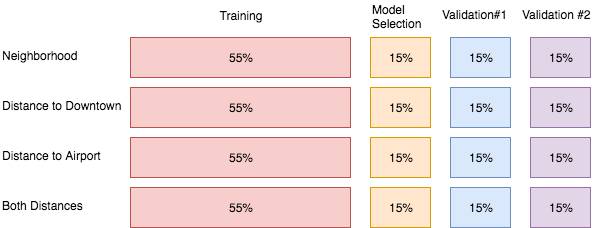
\includegraphics[width=0.7\textwidth]{data_separation.png}
            		\end{figure}
             
             
             \paragraph{(7) Choose Learning Methods:}
             	To investigate our questions, we use and compare the performance of three different supervised machine learning techniques: Linear Regression,Generalized Additive Models (GAMs), and Regression Trees.
             
             
             \paragraph{(8) Apply Methods:}
             	For each method, we apply the technique to each of the data transformations. The methods are trained on the training sets, and the model selection sets are used to select the best model within a method.
             
             \paragraph{(9) Compare Results:}
             	The best model of each method/transformation combination is evaluated on validation set \#1, and the root of the mean square error is obtained. At this point, we now have enough information to analyze the effects of replacing the ``neighborhood" feature with our chosen distance metrics.
               
             \paragraph{(10) Validate best Transformation/Method Combination:}
             	The method/transformation combination which has the least mean squared error on validation set \#1 is evaluated on validation set \#2. This ensures that we have a quality estimate of performance without overfitting, and we can now analyze the extent to which these methods can assist a host in determining the listing price for a property.


    	\subsection{Application of Methods}
            \subsubsection{Linear Regression}
            	\paragraph{}
                All linear regression models are applied on the set of datasets containing dummy variables for categorical variables. We choose to apply both LASSO and RIDGE regularization methods and finally compare their results.Both LASSO and RIDGE regularizes the model by penalizing the fitting of too many variables. LASSO model also allows us to do reduce dimensionality via regularization by shrinking the coefficients of a few variable  to 0, which essentially results in those variables having no effect on our model. Thus, reducing dimensionality and increasing interpretability and prediction accuracy. In theory, LASSO should give us a better accuracy in our case.
                
                Both parameters - lambda and number of predictors for both approaches are gathered using cross validation. The results are shared below.
                
            \subsubsection{Generalized Additive Models}
            	\paragraph{}
                GAMs provide a framework for extending the linear models explored above by representing each predictor as a non-linear function, while maintaining additivity. This approach was explored to investigate if representing continuous features with more degrees of freedom in combination with discrete features would result in a better results.
                \paragraph{}
                Each continuous predictor was represented by a Penalized Cubic regression spline$^{[4]}$. Smoothness selection was performed my maximum likelihood estimation using Restricted Maximum Likelihood (REML). For variable selection, three methods were performed: Regression Subset Selection and Forward Selection on a linear model with all predictors, and a shrinkage method within the GAM itself$^{[5]}$. The third method produced the best results on the model selection dataset. Essentially, there are smoothness penalties for each predictor, which include a small shrinkage component, so that for large enough smoothing parameters the smooth becomes identically zero.

            \subsubsection{Regression Trees}
            	\paragraph{}
                	% draft
                	When using tree-based methods, there are choices to be made for the tradeoff between interpretability and performance. Specifically, traditional regression trees have highly interpretable results whereas random forest and boosting methods trade interpretability for better performance. For our purposes, interpretability has relatively low importance, as (1) hosts will not change the features of their properties (e.g., changing the number of bedrooms), and (2) comparing data transformations involves comparing only the end results. Therefore, we choose to use boosting trees in our analysis.
             	\paragraph{}
                	For the parameters of our boosting trees, we select a tree depth of 1 and $\lambda = 0.001$. The number of trees is selected with cross-validation with a result of 10,000 trees.  
        
    
    
    \section{Results}
    % Show the results of your analysis. Summarize the results with a small number of most important figures or tables, and keep the description short.
    \subsection{Intermediate Results}
    	\subsubsection{Data Analysis}
        	\paragraph{}
            	The figure below shows the prices of each Airbnb listing before removal of outliers, with the orange line being the 95th percentile we used as the cutoff.
                
                \begin{figure}[H]
                	\centering
                	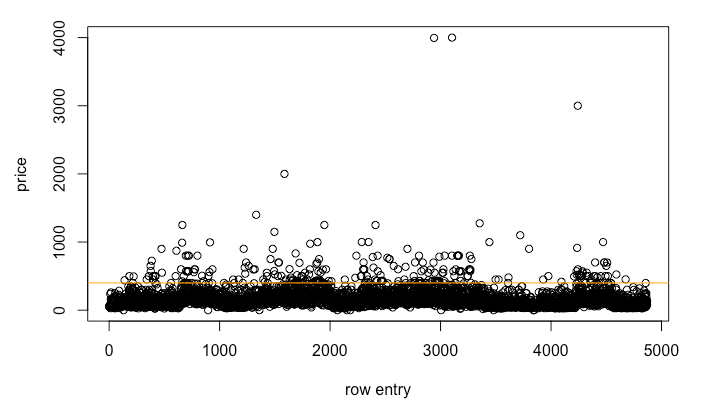
\includegraphics[width=0.6\textwidth]{outliers.png}
                \end{figure}
                
        	\paragraph{}
            	In the table below are statistics for price after removing outliers.
            	\begin{table}[H]
\centering
                \label{my-label4}
                \resizebox{0.7\textwidth}{!}{
                \begin{tabular}{l|l|l|l|l|l|l}
                       Min & 1st Qu. & Median & Mean & 3rd Qu. & Max & Standard Deviation\\ \hline
                \$0.0  & \$80.0      & \$133.0 & \$ 148.8 & \$199.0 & \$400.0 & \$84.6
                \end{tabular}}
                \end{table}
            
        	
            
    
    	\subsubsection{Linear Regression}
        	\paragraph{}
            We see that the MSE for LASSO regression were the least for all 4 datasets. However, the dataset containing neighborhood data gave us the best results with Lasso. The results from Model Selection dataset are as below:
            \begin{table}[H]
\centering

\label{my-label3}
\resizebox{0.5\textwidth}{!}{
\begin{tabular}{l|l|l|l}
       Dataset & $\lambda$ & \#Predictors & RMSE(\$) \\ \hline
Neighborhood  & 0.053       & 63             & 56.25        \\
Distance to Downtown & 0.16     & 40             & 59.17            \\
Distance to Airport  & 0.21         & 40             & 60.42           \\
Both & 0.11     & 41              & 58.62
\end{tabular}}
\end{table}
        
        \subsubsection{GAMs}
        	\paragraph{}
            GAM have the best results on the original dataset with `neighborhood` as a predictor. Evaluation was performed on the model selection dataset as shown in the table below. The square root of the mean-squared error obtained on the validation set \#1 was 55.75. The most significant predictors of `price` were: `neighborhood`, `property\_type`, `room\_type`, `instant\_bookable`, `accommodates`, `bedrooms`, `guests\_included`.'
           
		\begin{table}[H]
		\centering

			\label{my-label3}
			\resizebox{0.4\textwidth}{!}{
			\begin{tabular}{l|l}
       			Dataset & RMSE(\$) \\ \hline
				Neighborhood  & 55.15        \\
				Distance to Downtown & 58.05            \\
				Distance to Airport  & 56.24           \\
				Both & 55.77
\end{tabular}}
\end{table}
        
        \subsubsection{Regression Trees}
        	\paragraph{}
            	The relative importance of the four most important variables for each transformation are shown in the table below.
            \begin{table}[H]
\centering

\label{my-label2}
\resizebox{\textwidth}{!}{
\begin{tabular}{l|ll|ll|ll|ll}
       & NVar & NRel & DDVar & DDRel & DAVar & DARel & DBVar    & DBRel \\ \hline
First  & room\_type       & 46.9             & room\_type    & 50.6          & room\_type   & 51.7         & room\_type   & 50.1      \\
Second & neighborhood     & 20.3             & bedrooms      & 15.7          & dairport     & 15.7         & bedrooms     & 15.8      \\
Third  & bedrooms         & 15.7             & ddowntown     & 15.1          & bedrooms     & 15.1         & ddowntown    & 11.5      \\
Fourth & accommodates     & 7.7              & accommodates  & 8.1           & accommodates & 8.2          & accommodates & 7.9      
\end{tabular}}
\end{table}
            
	\subsection{Final Results}
    	\paragraph{}
        	The square root of the mean squared error of each transformation/method combination on validation set \#1 is shown in the figure below.
        	\begin{table}[H]
              \centering
              \caption{Square Root of the MSE}
              \label{my-label}
              \begin{tabular}{l|llll}
                                     & Linear Regression & GAM & Regression Trees &  \\ \cline{1-4}
                Neighborhood         & 56.82             &  55.15   &    55.75     &  \\
                Distance to Downtown & 58.95             &  58.05   &    57.00   &  \\
                Distance to Airport  & 60.76             &  56.24   &    56.57   &  \\
                Both Distances       & 58.16             &  55.77   &    56.54     & 
              \end{tabular}
            \end{table}
            
        \paragraph{}
        	The transformation/method combination with the best performance was the dataset with the ``neighborhood" feature using the GAM method. This transformation/method combination was tested on validation set \#2, and the square root of the mean squared error was 52.30.
    
    \section{Discussion}
    % What did you learn from this analysis? What additional steps could be potentially performed to improve your analysis?
    \subsection{Answers to Project Questions}
    	\subsubsection*{(1) Performance}
        	\paragraph{}
            	The root of the mean squared error of our best model/transformation combination was \~50. Considering that the median price is \$133 with a standard deviation of \$84 , this result is useful but not exceptional. These methods can be used to give an Airbnb host a rough estimate of the price to charge, but it is clear that there is important information not captured by the features we used.
            
         \subsubsection*{(2) Data Transformation Feasibility}
         	\paragraph{}
            	The performance results after replacing the ``neighborhood" feature with driving distance to a geographic point of interest were nearly identical to the performance results on the original data. This result raises the concern that the ``neighborhood" feature is actually non-informative, and thus transforming it will not have an impact. However, we see in our intermediate analysis that the ``neighborhood" and transformed features are consistently in the most influential features as reported by the methods used. Therefore the transformation of the ``neighborhood" feature is nontrivial, and our results are evidence that the information captured by this feature can be reasonably represented as distance to some location of importance. 
    
    \subsection{Improvements and Further Research}
    	\paragraph{}
        	There are several ways the work presented in this paper could be expanded. In our analysis, we did not utilize any of the textual features in the original dataset, as this would require techniques outside the scope of the course. However, it is likely that the textual features contain useful information for predicting price, and NLP techniques such as sentiment analysis could be used to include these features and increase performance.
        \paragraph{}
        	Additionally, we selected the geographic points of interest using our intuition regarding what locations would be relevant for pricing. A more sophisticated process could be developed for selecting points of interest to consider.
    
    
    \pagebreak
    \section{References}
    % Please only add references that are explicitly used in the text. Make sure that you cite the sources of data, and the associated publications. Use consistent format and numbering scheme.
    
    \paragraph{}
    		\begin{description}
            	\item[(1)] \url{http://insideairbnb.com/about.html}
                \item[(2)] \url{http://insideairbnb.com/get-the-data.html}
                \item[(3)] \url{https://cran.r-project.org/web/packages/gmapsdistance/gmapsdistance.pdf}
                \item[(4)] \url{https://stat.ethz.ch/R-manual/R-devel/library/mgcv/html/smooth.construct.cr.smooth.spec.html}
                \item[(5)] \url{https://stat.ethz.ch/R-manual/R-devel/library/mgcv/html/gam.selection.html}
            \end{description}
    
    
\end{document}
